\section{Cấu trúc và các góc nhìn kiến trúc}
\label{sec:architecture-views}

\subsection{Module view}
\label{subsec:module-view}
Các module nghiệp vụ và trách nhiệm được tổng hợp tại Bảng~\ref{tab:services}. Bảng thể hiện ranh giới sở hữu nghiệp vụ; mức độ hoàn thiện endpoint được đánh giá riêng theo mã nguồn. Các service Java tổ chức các package controller, service, entity, repository, DTO, config, client và messaging tùy theo nhu cầu triển khai. Mỗi service có POM độc lập.

\begin{table}[htbp]
\centering
\caption{Các service nghiệp vụ và kho dữ liệu sở hữu}\label{tab:services}
\begin{tabular}{|>{\raggedright\arraybackslash}p{0.25\linewidth}|>{\raggedright\arraybackslash}p{0.43\linewidth}|>{\raggedright\arraybackslash}p{0.22\linewidth}|}\hline
\textbf{Service} & \textbf{Trách nhiệm chính} & \textbf{Kho dữ liệu} \\\hline
Identity \& User & Nhân viên, tài khoản, OAuth2, vai trò và quyền nhà máy & PostgreSQL \\\hline
QR & Phát hành, ký, xác minh, thu hồi và redemption credential & PostgreSQL \\\hline
Gate Station & Nhà máy, trạm, cấu hình, danh tính thiết bị và adapter cổng & PostgreSQL \\\hline
Access Event & Scan, chính sách truy cập, command, confirmation, passage và review bằng chứng muộn & PostgreSQL \\\hline
Attendance Report & Inbox passage, tính công, điều chỉnh, snapshot kỳ & PostgreSQL \\\hline
HR Integration & Batch export, attempt, receipt, retry và reconciliation & PostgreSQL \\\hline
Audit \& Notification & Audit sự kiện và công việc thông báo & MongoDB \\\hline
\end{tabular}
\end{table}

Hạ tầng gồm API Gateway bảo vệ/định tuyến API, Eureka làm registry và Config Server cung cấp cấu hình. Gateway và các service xác minh JWT theo OAuth2 Resource Server; Identity cấp token. Scope JWT được ánh xạ sang authority \texttt{SCOPE\_*}. Quyền theo vai trò và nhà máy được kiểm tra thêm tại service nghiệp vụ.

\subsection{Component-and-connector view}
\label{subsec:connector-view}
Hình~\ref{fig:runtime-flow} mô tả luồng thực thi chính và các ranh giới tích hợp với policy adapter, turnstile. Trong mã nguồn Access Event, REST controller tiếp nhận scan/callback; ca sử dụng \texttt{AccessService} phụ thuộc vào các abstraction \texttt{AccessPolicy}/\texttt{AccessStore}, các adapter persistence và outbox publisher. \texttt{GateSimulator} phục vụ kiểm chứng hợp đồng mô phỏng, không đại diện cho adapter phần cứng turnstile.

\begin{figure}[htbp]
\centering
\resizebox{\textwidth}{!}{%
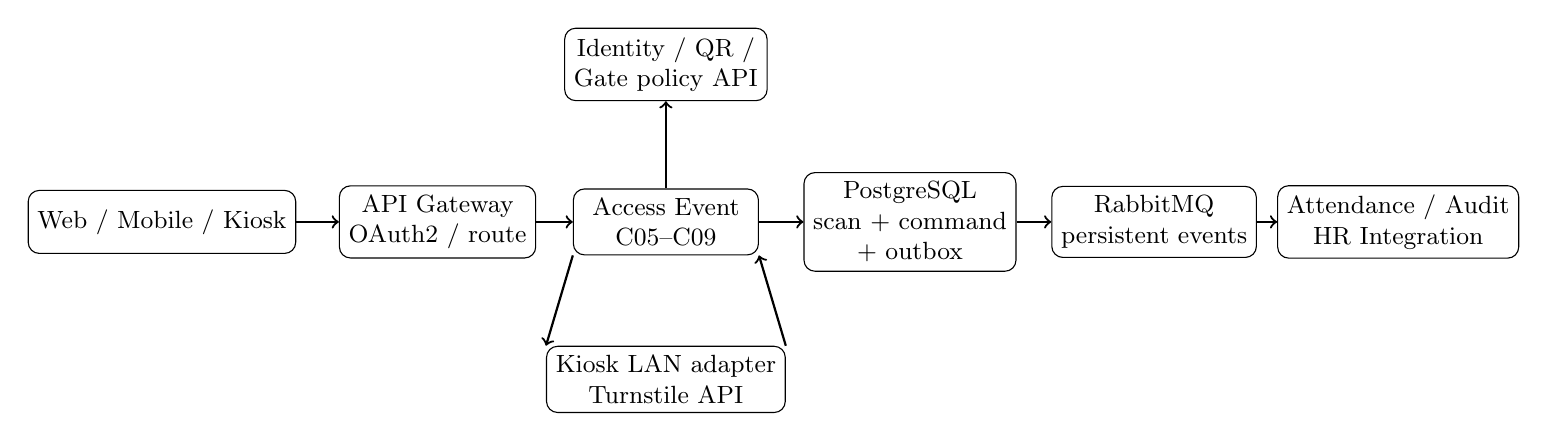
\begin{tikzpicture}[node distance=0.75cm and 0.8cm, box/.style={draw, rounded corners, align=center, minimum width=2.35cm, minimum height=0.8cm, font=\small}, arr/.style={->, thick}]
\node[box] (client) at (0,0) {Web / Mobile / Kiosk};
\node[box] (gateway) at (3.5,0) {API Gateway\\OAuth2 / route};
\node[box] (access) at (6.4,0) {Access Event\\C05--C09};
\node[box] (policy) at (6.4,2.0) {Identity / QR /\\Gate policy API};
\node[box] (turnstile) at (6.4,-2.0) {Kiosk LAN adapter\\Turnstile API};
\node[box] (db) at (9.5,0) {PostgreSQL\\scan + command\\+ outbox};
\node[box] (mq) at (12.6,0) {RabbitMQ\\persistent events};
\node[box] (consumers) at (15.7,0) {Attendance / Audit\\HR Integration};
\draw[arr] (client.east)--(gateway.west);
\draw[arr] (gateway.east)--(access.west);
\draw[arr] (access.north)--(policy.south);
\draw[arr] (access.east)--(db.west);
\draw[arr] (access.south west)--(turnstile.north west);
\draw[arr] (turnstile.north east)--(access.south east);
\draw[arr] (db.east)--(mq.west);
\draw[arr] (mq.east)--(consumers.west);
\end{tikzpicture}
}%
\caption{Luồng runtime của yêu cầu scan và truyền sự kiện bất đồng bộ}
\label{fig:runtime-flow}
\end{figure}

Đường đồng bộ thực hiện xác thực, đánh giá policy và ghi trạng thái bền vững. Kết quả tới cổng được xác nhận riêng; \texttt{ALLOW}, cổng báo \texttt{OPENED} và người thực sự \texttt{PASSED} là các bằng chứng khác nhau. Chỉ passage được xác nhận/duyệt mới được chiếu sang Attendance. Event được consumer nhận theo at-least-once, dedup theo event ID và ACK sau commit. Không tuyên bố exactly-once qua ranh giới broker.

\subsection{Allocation view}
\label{subsec:allocation-view}
Hình~\ref{fig:allocation} thể hiện phương án phân bổ triển khai dự kiến. Backend hiện được phát triển và chạy trong môi trường cục bộ với các dependency cấu hình riêng; sơ đồ chưa phản ánh topology production đã nghiệm thu. Trong phương án vận hành, kiosk tại hai nhà máy gọi backend qua HTTPS, còn adapter thiết bị giao tiếp với turnstile trong mạng LAN. Tầng ứng dụng có thể triển khai nhiều instance trên các máy chủ độc lập; database và broker được cô lập trong mạng riêng. Config Server/Eureka cần cấu hình HA tương ứng; database cần backup, replication và quy trình failover có kiểm soát split-brain.

\begin{figure}[htbp]
\centering
\resizebox{\textwidth}{!}{%
\begin{tikzpicture}[node distance=0.7cm and 1.0cm, box/.style={draw, rounded corners, align=center, minimum width=2.6cm, minimum height=0.8cm, font=\small}, arr/.style={->, thick}]
\node[box] (bd) {Nhà máy Bình Dương\\Kiosk + cổng quay};
\node[box, below=of bd] (la) {Nhà máy Long An\\Kiosk + cổng quay};
\node[box, right=of bd, yshift=-0.4cm] (lb) {HTTPS Load Balancer\\(dự kiến)};
\node[box, right=of lb] (app) {Gateway + services\\nhiều instance};
\node[box, right=of app] (data) {PostgreSQL theo service\\MongoDB + RabbitMQ};
\node[box, above=of app] (infra) {Config Server + Eureka};
\node[box, below=of data] (hr) {HR/Payroll API\\email/notification};
\draw[arr] (bd)--(lb);
\draw[arr] (la)--(lb);
\draw[arr] (lb)--(app);
\draw[arr] (infra)--(app);
\draw[arr] (app)--(data);
\draw[arr] (data)--(hr);
\end{tikzpicture}
}%
\caption{Allocation view triển khai dự kiến; HA chưa được nghiệm thu}
\label{fig:allocation}
\end{figure}

\subsection{Quyết định kiến trúc}
\label{subsec:adrs}
\begin{table}[htbp]
\centering
\caption{Các quyết định kiến trúc ảnh hưởng trực tiếp tới lát cắt C05--C09}\label{tab:adrs}
\begin{tabular}{|>{\raggedright\arraybackslash}p{0.12\linewidth}|>{\raggedright\arraybackslash}p{0.35\linewidth}|>{\raggedright\arraybackslash}p{0.43\linewidth}|}\hline
\textbf{ADR} & \textbf{Quyết định} & \textbf{Hệ quả/đánh đổi} \\\hline
ADR-01 & Bảy service nghiệp vụ Java; ba ứng dụng hạ tầng & Tách ownership và triển khai; tăng chi phí mạng, cấu hình và vận hành. \\\hline
ADR-02 & Database logic riêng theo service; không đọc/ghi chéo & Giảm coupling dữ liệu; cần API/event và nhất quán cuối cùng. \\\hline
ADR-03 & QR ký số, thời hạn ngắn; Access kiểm soát redemption & Giảm tái sử dụng và replay; cần bảo vệ khóa, đồng bộ giờ và chính sách thu hồi. \\\hline
ADR-04 & Event append-only, transactional outbox/inbox & Tránh mất event khi broker gián đoạn; chấp nhận giao trùng và cần dedup. \\\hline
ADR-05 & Quyết định tập trung; kiosk gọi cổng qua adapter LAN & Không có offline authorization tại nhà máy; outage cần quy trình ngoại lệ có audit. \\\hline
ADR-06 & Tách command, confirmation và passage & Không tính công từ quyết định cho phép hay tín hiệu mở cổng; phụ thuộc bằng chứng thiết bị. \\\hline
ADR-07 & OAuth2 API, danh tính thiết bị gắn với station & Hạn chế giả mạo scope/site; cần quy trình cấp/thu hồi credential. \\\hline
\end{tabular}
\end{table}

Các nguyên tắc thiết kế là phân tách trách nhiệm; fail closed khi không xác minh được quyền; idempotency với ID ổn định; append-only cho bằng chứng; least privilege; giảm PII trong event; contract-first cho API/event; và giám sát backlog, DLQ, độ trễ HR. Outbox/inbox và UNKNOWN biểu diễn lỗi như trạng thái nghiệp vụ cần phục hồi, không che lấp bằng retry vô hạn.

